\documentclass[floatfix,superscriptaddress,a4paper,twocolumn]{revtex4-1}
\usepackage[T1]{fontenc}
\usepackage{lmodern}
\usepackage[utf8]{inputenc}
\usepackage{amsmath}
\usepackage{amssymb}
\usepackage{paralist}
\usepackage{booktabs}
\usepackage{tabularx}
\usepackage[version=3]{mhchem}
\usepackage{wrapfig}
\usepackage{pifont}
\usepackage{mathrsfs}
\usepackage{tikz}
\usepackage{xcolor}
\usepackage{color}
\usepackage{enumitem}
\usepackage{datetime}
\usepackage{textcomp}
\usepackage{relsize}
%\setlist{noitemsep}
\usepackage{lineno}
%\linenumbers

\usepackage{pgfplots}
\pgfplotsset{compat=newest}
\usepgfplotslibrary{units}
\usetikzlibrary{pgfplots.units}
\usetikzlibrary{calc}
\usepackage{siunitx}
\sisetup{ per-mode = reciprocal }
%\DeclareSIUnit\molar{\mole\per\cubic\deci\metre}
%\DeclareSIUnit\textsc{M}{\textsc{M}}
\DeclareSIUnit\particle{particle}
\DeclareSIUnit\g{g}

\usepackage{hyperref}
\hypersetup{
	colorlinks=false,
	hidelinks=true,
	pdfauthor={Aaron Webster},
}

\newcommand{\Figure}[1]{FIG.~\ref{#1}}
\newcommand{\Figures}[2]{FIG.~\ref{#1}~and~\ref{#2}}
\newcommand{\Equation}[1]{EQN.~\ref{#1}}
\newcommand{\Table}[1]{TBL.~\ref{#1}}
\newcommand{\Section}[1]{SEC.~\ref{#1}}
\newcommand{\Chapter}[1]{CH.~\ref{#1}}
\newcommand{\Appendix}[1]{APPENDIX~\ref{#1}}

% use roman type for natural base e and sqrt(-1)
\newcommand{\me}{{\mathrm{e}}}
\newcommand{\mi}{{\mathrm{i}}}

% New definition of square root:
% it renames \sqrt as \oldsqrt
% This definition puts a little vertical guy at the end so it's more
% obvious where the square root actually ends.
\let\oldsqrt\sqrt
% it defines the new \sqrt in terms of the old one
\def\sqrt{\mathpalette\DHLhksqrt}
\def\DHLhksqrt#1#2{%
\setbox0=\hbox{$#1\oldsqrt{#2\,}$}\dimen0=\ht0
\advance\dimen0-0.2\ht0
\setbox2=\hbox{\vrule height\ht0 depth -\dimen0}%
{\box0\lower0.4pt\box2}}

\definecolor{colora}{RGB}{24,90,169}
\definecolor{colorb}{RGB}{238,46,47}
\definecolor{colorc}{RGB}{0,140,72}
\definecolor{colord}{RGB}{244,125,35}
\definecolor{colore}{RGB}{61,90,153}
\definecolor{colorf}{RGB}{102,44,145}
\definecolor{tangoorange}{RGB}{245,121,0}

\newcommand{\df}{\Delta\!f}
\newcommand{\dg}{\Delta\Gamma}
\newcommand{\xil}{\xi_\mathrm{L}}
\newcommand{\kl}{k_\mathrm{L}}
\newcommand{\ml}{m_\mathrm{L}}
\newcommand{\kq}{k_\mathrm{q}}
\newcommand{\mq}{m_\mathrm{q}}
\newcommand{\omegaq}{\omega_\mathrm{q}}

\newcommand{\todo}[1]{%
\textcolor{tangoorange}{#1}
}

\begin{document}

\title{Probing biomechanical properties with a centrifugal force quartz crystal microbalance}
\author{Aaron~Webster}
\email{aaron.webster@mpl.mpg.de}
\affiliation{Max Planck Institute for the Science of Light, Günther-Scharowsky-Str. 1/Bau 24, Erlangen D-91058, Germany}
\author{Frank~Vollmer}
\affiliation{Max Planck Institute for the Science of Light, Günther-Scharowsky-Str. 1/Bau 24, Erlangen D-91058, Germany}
\author{Yuki~Sato}
\affiliation{The Rowland Institute at Harvard, Harvard University, 100 Edwin H. Land Boulevard, Cambridge, Massachusetts 02142, USA}

%\tikz[overlay,remember picture] {
% \node at ($(current page.west)+(1,0)$) [rotate=90]
% {\large\textcolor{gray}{\input{commithash} \pdfdate}};
%}

\begin{abstract}
  Application of force on biomolecules has been instrumental in understanding
  biofunctional behavior from single molecules to complex collections of
  cells.  Current approaches, for example those based on atomic force
  microscopy or magnetic or optical tweezers, are powerful but limited in
  their applicability as integrated biosensors.  Here we describe a new
  force-based biosensing technique based on the quartz crystal microbalance.
  By applying centrifugal forces to a sample, we show it is possible to
  repeatedly and non-destructively interrogate its mechanical properties \textit{in situ}
  and in real time.  We employ this platform for the studies of
  micron-sized particles, viscoelastic monolayers of DNA, and particles
  tethered to the quartz crystal microbalance surface by DNA\@.  Our results indicate that, for certain types
  of samples on quartz crystal balances, application of centrifugal force both enhances sensitivity and
  reveals additional mechanical and viscoelastic properties.
\end{abstract}

\date{\today}
\maketitle

\section*{Introduction}
\label{sec:introduction}
There are few experimental techniques that allow the
study of force on biological molecules.  Among
them, optical or magnetic tweezers and atomic force microscopes (AFMs) have
provided much insight into the mechanics of DNA, RNA and
chromatin~\cite{felsenfeld1992chromatin}~\cite{cui2000pulling}~\cite{larson2012trigger}~\cite{marko1995stretching},
friction and wear in
proteins~\cite{suda2001origin}~\cite{bormuth2009protein} and stepwise
motion of motor proteins~\cite{asbury2003kinesin}, all of which are
important for understanding disease.  However powerful, these methods have
difficulty operating as integrated devices to probe the mechanical
properties of heterogeneous samples in a wide range of applications
\textit{in situ} and in real time; tweezer and AFM experiments rely on
highly trained experimentalists, are not widely applicable as analytical
tools, and are often constrained to the analysis of well prepared,
homogeneous samples.

Among direct mechanical transduction methods amenable for biosensing, the
quartz crystal microbalance (QCM) has seen great utility as a simple, cost
effective, and highly versatile mechanical biosensing platform.  Since its
introduction by Sauerbrey~\cite{sauerbrey1959verwendung} in 1959 as a
thin-film mass sensor in the gas phase, the understanding and real-world
applicability of these devices has been repeatedly enhanced
to study phenomena such as viscoelastic films in the liquid
phase~\cite{kanazawa1985frequency}, contact
mechanics~\cite{johannsman2007contacts}, and complex samples of biopolymers
and biomacromolecules~\cite{marx2003quartz}.

Naturally, these benefits do not come without disadvantages. The
underlying mechanical properties of the sample that occur upon loading of
the biomaterial are often not revealed by the stepwise changes in the QCM
sensorgram, an issue complicated by the choice of theoretical model.

Here we introduce a novel \gls{qcm}.based biosensing technique which enables
monitoring the mechanical response of a sample to the continuous
application of a variable centrifugal force.  This centrifugal force quartz
crystal microbalance (CF-QCM) concept enables direct introduction of pico-
to nanoscale forces in the liquid phase for analyzing a sample's mechanical
properties.  We show that the response of a sample under
centrifugal load is revealing of its viscoelastic, mechanical, and conformal
properties.
\begin{figure*}[ht]
  \centering
  %\includegraphics[]{Figure-1_webster.pdf}
  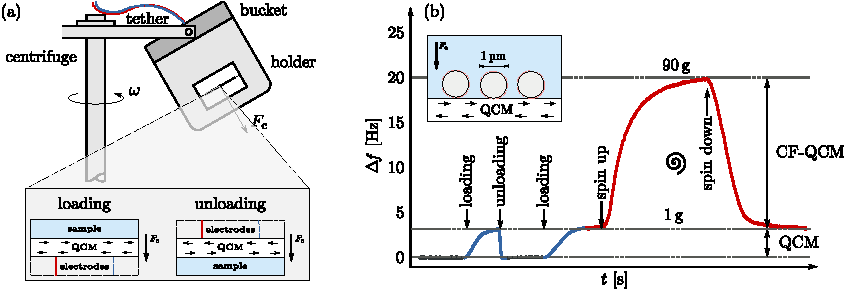
\includegraphics{figure1.pdf}
  \caption{Overview of the CF-QCM\@.  (a) Experimental setup.  A \gls{qcm} and its driver are integrated into one
    arm of a standard swinging bucket centrifuge.  Data acquisition is done
    electrically through a tether and a centrally mounted slip ring.  When
    spinning, centrifugal force is applied to a sample under assay. Here
    $F_\mathrm{c} \equiv m \sqrt{a_\mathrm{c}^2 +a_\mathrm{g}^2}$, where
    $a_\mathrm{c}=\omega^2 R$ and $a_\mathrm{g}$ are centripetal and gravitational
    accelerations, respectively.  (b)
    Example CF-QCM experiment with \SI{1}{\micro\meter} particles in water,
    $N_\mathrm{L}=\SI{1.58e11}{\particle\per\meter\squared}$, in the
    ``loading'' configuration (inset).  The horizontal arrows indicate the
    motion of the \gls{qcm}['s] transverse shear mode.
    The spin up to \SI{90}{g} in
    loading configuration enhances the \gls{qcm} frequency shift signal and allows
    extraction of mechanical properties of the sample, as well as particle
    size. See text for details.
  }
  \label{fig:expsetup}
\end{figure*}


\section*{Results}
\label{sec:experiment}
\subsection*{Experiment}
The experimental setup under consideration is shown schematically in
\Figure{fig:expsetup}(a).  It consists of a \gls{qcm} integrated into the arm of
a commercial swinging bucket centrifuge.  The \gls{qcm} is connected in proximity
to a remote driver which is tethered via a slip-ring connector to external
data acquisition electronics.  The crystal itself is mounted in a holder
radially by its edges such that the centrifugal force $F_\mathrm{c}$ is
always normal to the surface of the crystal.  On the sensing side of the
crystal is a $\SI{125}{\micro\liter}$ volume PDMS/glass cell containing the
sample.  The non-sensing side of the crystal remains in air.
\linelabel{line:xtalorientation}When in
operation, the crystal and cell are mounted in either the \textit{loading}
configuration, where the centrifugal force is \textit{in to} the sensing
side or, by mounting it upside down, in the \textit{unloading}
configuration, where the force is \textit{away from} the sensing side.

An example CF-QCM response for free particles is depicted to the left in
\Figure{fig:expsetup}(b).  Here, free \SI{1}{\micro\meter} streptavidin
coated polystyrene particles in water are introduced into the sample cell.
When the cell is rotated to the loading configuration under the influence
of gravity alone, the particles fall toward the sensing surface and a positive
shift in the \gls{qcm}['s] frequency signal is observed.  When the cell is then
rotated 180 degrees to the unloading configuration, the particles fall off
and the frequency response returns to its original state.  Again the cell
is rotated 180 degrees to the loading configuration and the positive
frequency shift is observed.  As the centrifuge spins up towards
\SI{90}{g}, the particles are ``pressed'' towards the \gls{qcm} surface and a
four fold increase in the frequency shift is observed.  The centrifuge then
spins down and the baseline frequency shift under gravity alone is
recovered.

Traditional \gls{qcm} experiments assume that the inertial properties and
rigidity of the sample's coupling are taken as a fixed parameter (or
statistical distribution) under assay.  With this approach however, one is
only able to obtain discrete values in an otherwise continuous parameter space.  Hybrid-QCM experiments
involving nanoindenters~\cite{borovsky2001measuring} or AFM probe
tips~\cite{richter2003pathways} have shown intriguing behavior when force
is applied to a sample in a \gls{qcm} measurement.  \linelabel{line:accreport}There have also been reports
that accelerations as small as \SI{1}{g} have a measurable effect on a
QCM's response for viscoelastic monolayers such as
DNA~\cite{fawcett2004evidence}, and even for pure Newtonian
liquids~\cite{yoshimoto2002effect}.  All of these responses have been found
to be significant compared to the baseline acceleration sensitivity of the
QCM itself~\cite{filler1988acceleration}.  With the integration of a
centrifuge to a standard \gls{qcm}. one can observe these effects under enhanced
g-forces and make endpoint measurements (measurements taken after the
addition of a sample) in the sample's parameter space continuously and
repeatedly.

To demonstrate this, we have examined six different samples in the CF-QCM
under variable accelerations from approximately \SIrange{1}{90}{g}.  These
samples were chosen to be examples of the breadth of load situations
accessible with our technique.  They are:
\begin{inparaenum}[(a)]
  \item air,
  \item deionized water,
  \item free particles in water,
  \item paramagnetic particles attached to the sensor via short oligonucleotides,
  \item \SI{48}{kbp} lambda phage DNAs attached to the gold electrode, and
  \item polystyrene particles tethered to the sensor via \SI{48}{kbp} lambda phage DNAs.
\end{inparaenum}

\linelabel{line:qcmbvd}The employed \gls{qcm} driver circuit outputs Butterworth van Dyke (BvD)
equivalent relative frequency $\df$ (in hertz) and motional resistance $R$ (in ohms).
$R$ is approximately related to the bandwidth $\Gamma$ (half width at half
maximum of the frequency response) by $\Gamma=R/\left(4\pi L\right)$, where
$L=\SI{40}{\milli\henry}$ is the motional inductance of the BvD
equivalent circuit~\cite{arnau2002circuit}.  For this
relationship we assume the small load approximation $\df/f_\mathrm{F} \ll
  1$, where $f_\mathrm{F}$ is the fundamental frequency~\cite{geelhood2002transient}.
\linelabel{line:bandwidthdev}It is therefore relevant to note our assumption that $\Delta R$ is an
approximate, and indirect, measure of the bandwidth $\dg$ (in
hertz).  In addition $\dg$ is an equivalent representation of the ``dissipation'', $D$, used in
QCM-D devices by $D=2\dg/f_\mathrm{F}$ (See Supplementary Note 1).
\begin{figure*}[ht]
  \centering
  %\hspace{-1.0cm}
  %\includegraphics{Figure-3_webster.pdf}
  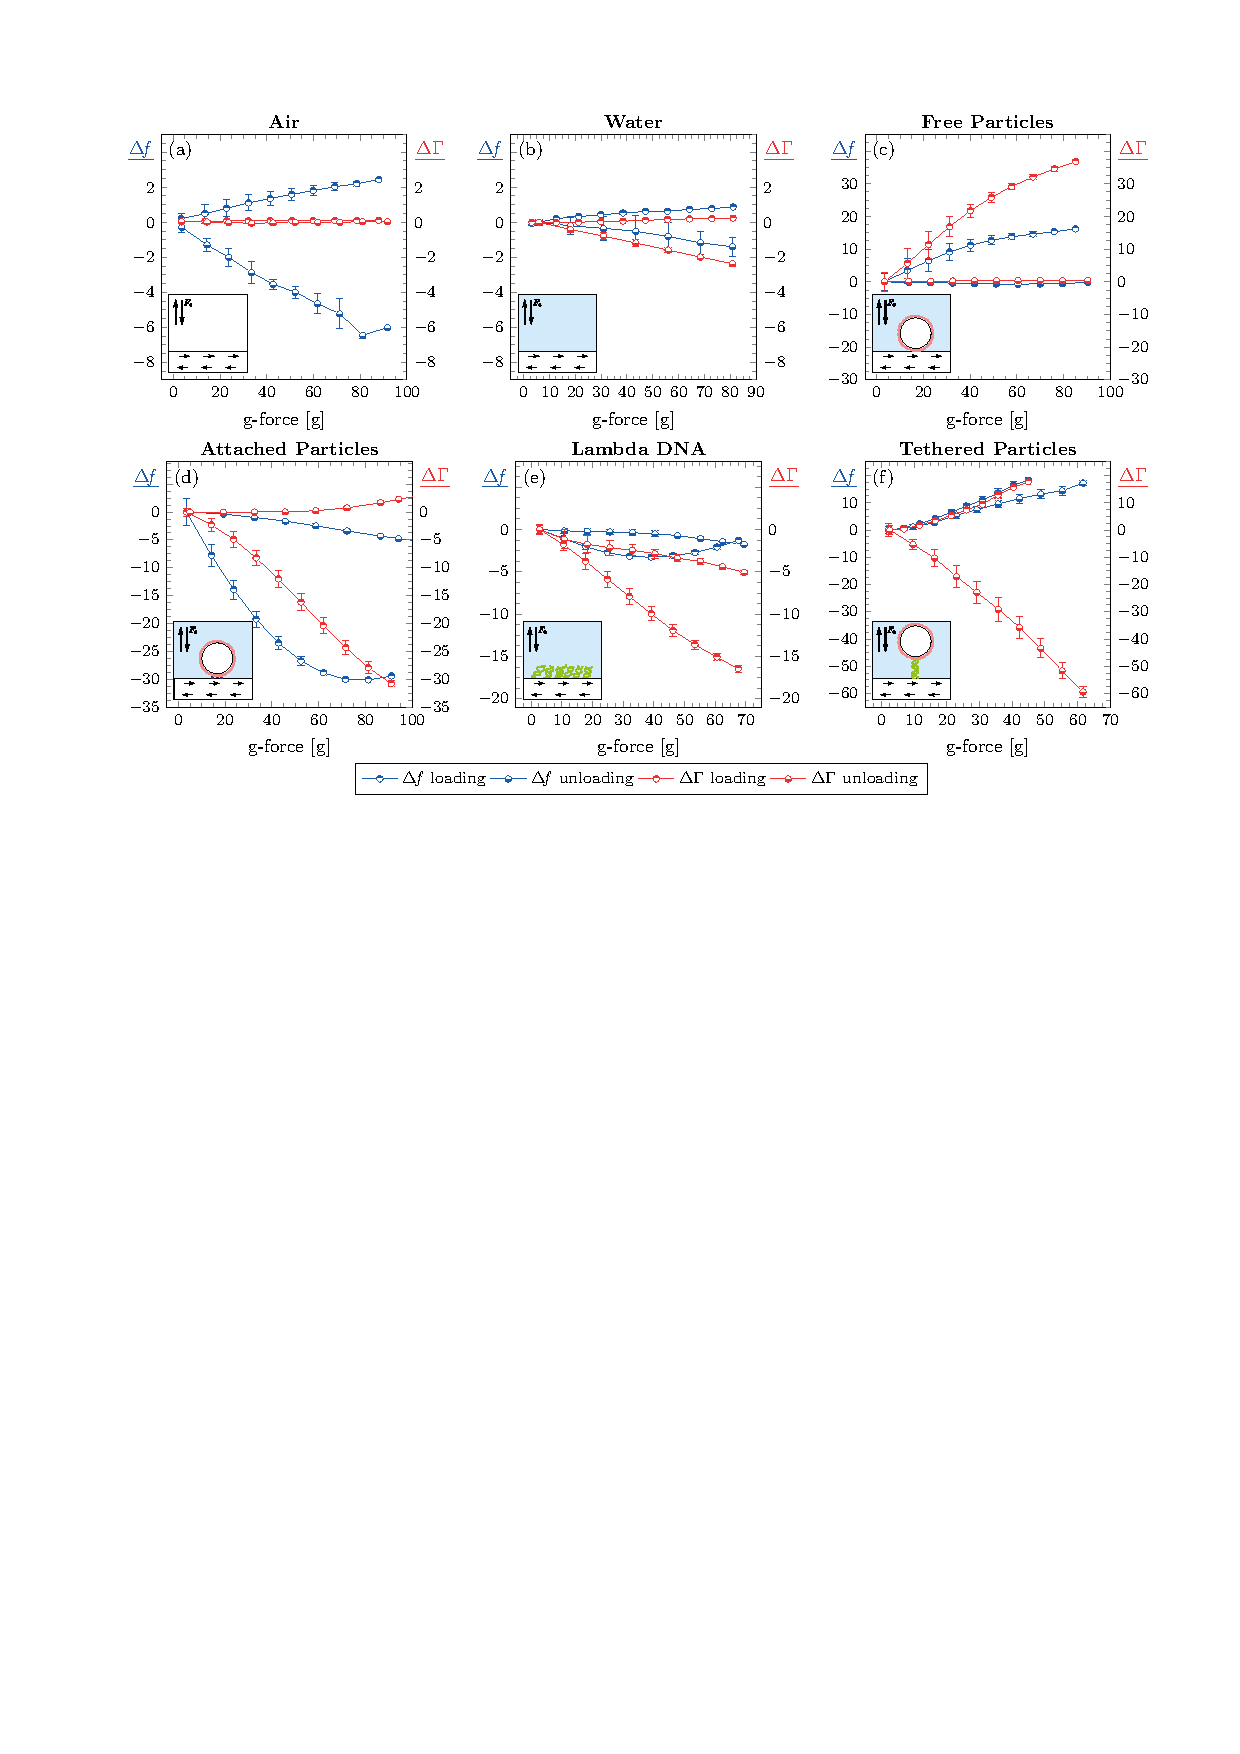
\includegraphics{figure2.pdf}
  \caption{Load situations.
    Change in frequency $\df$ and bandwidth $\dg$
    (in hertz, inferred from motional resistance) of
    the CF-QCM under different load situations as the centripetal acceleration
    is directed in to (\textit{loading}, represented by circles with the top half
    colored) and out of (\textit{unloading}, represented by circles with the
    bottom half colored) the plane of the crystal.
    The situations are
    (a) unloaded crystal in air,
    (b) deionized water,
    (c) free \SI{1}{\micro\meter} diameter streptavidin-coated polystyrene
    particles, $N_\mathrm{L}=\SI{1.58e11}{\particle\per\meter\squared}$,
    (d) \SI{2}{\micro\meter} diameter streptavidin-coated paramagnetic
    particles, $N_\mathrm{L}=\SI{1.65e10}{\particle\per\meter\squared}$,
    attached with \SI{25}{mer} oligonucleotides,
    (e) lambda DNA only attached to the gold electrode, and
    (f) \SI{25}{\micro\meter} diameter streptavidin
    coated polystyrene particles,
    $N_\mathrm{L}=\SI{3.25e7}{\particle\per\meter\squared}$, tethered to the sensor surface with
    \SI{48}{kbp} lambda DNAs.  Error bars are derived from uncertainties
    (standard deviation) in
    the centrifuge both spinning up and spinning down in a single experimental
    run.
  }
  \label{fig:loadplot}
\end{figure*}

The instrument's response was first tested in air, shown in
\Figure{fig:loadplot}(a).  \linelabel{line:dfdg}The base acceleration sensitivity (change in
frequency versus change in g-force) of AT cut quartz normal to the plane of
the crystal has a reported value~\cite{valdois2794influence} of $\df/\Delta
  g =\SI{2.188+-0.006e-2}{\hertz\per\g}$.  Our instrument shows similar behavior:
$\df/\Delta g =\SI{2.682+-0.023e-2}{\hertz\per\g}$ in the loading
configuration.  The signs of $\df/\Delta g$ are found to be opposite in the loading
and unloading configurations.  We have not found a reference for the
bandwidth or motional resistance dependence of a \gls{qcm} under acceleration,
but we find the value to be $\dg/\Delta g = \SI{9.203+-0.171e-4}{\hertz\per\g}$.

Next, deionized water was used as a control sample for measurement in the
liquid phase, as shown in \Figure{fig:loadplot}(b).  The initial shift in
frequency and bandwidth is in agreement with what is obtained the Kanazawa-Gordon
relations~\cite{kanazawa1985frequency} for water
($\rho=\SI{1}{\gram\per\centi\meter\cubed}$ and
$\eta=\SI{1}{\milli\pascal\second}$): $\df = \SI{-714}{\hertz}$ and
$R=\SI{359}{\ohm}$, which are close to the measured values of $\df =
  \SI{-716}{\hertz}$ and $R=\SI{357}{\ohm}$.  \linelabel{line:dfdgapart}The response under centrifugal
load was found to be linear and smaller than that of air: $\df/\Delta g=
  \SI{1.357+-0.024e-2}{\hertz \per\g}$ and $\dg/\Delta g=
  \SI{2.865+-0.073e-3}{\hertz\per\g}$.  We observe that these acceleration
dependent forces in the liquid phase are not necessarily commensurate with
those in the gas phase, but as the effects are small compared to
experiments with actual loads, we treat them as baselines to be
subtracted.

Utilizing the flexibility that the instrument provides in modifying the
coupling between the load and the sensor surface, we have applied the
technique to the study of discrete micron-sized particles.  As first
referenced in \Figure{fig:expsetup}(b), the frequency and bandwidth shifts
of free particles in the liquid phase as a function of g-force is shown in
\Figure{fig:loadplot}(c).  Here, streptavidin-coated polystyrene particles,
mean diameter $\bar{d}=\SI{1.07}{\micro\meter}$, are placed in the sample volume with
a surface density of
$N_\mathrm{L}=\SI{1.58e11}{\particle\per\meter\squared}$ and the signal is
observed in both the loading and unloading configurations.
\linelabel{line:particleattach}The particles
did not exhibit adhesion to either the unmodified gold electrode or the
glass/PDMS cell surrounding it; in the unloading configuration, the particles
quickly drifted away from the sensing area and a signal identical to water
was observed.  \linelabel{line:loadingpshift}In the loading configuration, a large positive
shift in $\df$ and $\dg$ was observed, consistent with
previously observed responses for weakly coupled particles in this size
range~\cite{johannsman2007contacts}.

The initial shift under \SI{1}{g} was found to be $\df=
  \SI{2.2}{\hertz}$ and $\dg=\SI{7.5}{\hertz}$.  At the maximum acceleration of \SI{90}{g} the
signal increases to $\df = \SI{16.5}{\hertz}$ and $\dg=\SI{37}{\hertz}$. This also
represents a sensitivity enhancement in the minimum resolvable surface
density of the particles.  The scaling of $\df$ and $\dg$ with increasing
centrifugal load is nonlinear in the applied load, implying non-Hertzian
behavior~\cite{borovsky2001measuring}.
%The exact mechanism of coupling and relation of the applied force with is
%beyond the scope of this manuscript.

The same experiment was also carried out with \num{2}, \num{6}, \num{15},
and \SI{25}{\micro\meter} polystyrene particles.
%(actual mean diameters $d=\bar{d}=1.89, 5.86,, 15\,\mathrm{and}\;\SI{24.8}{\micro\meter}$).
The loading curves all
followed the same trend, but the relative shifts in $\df$ and $\dg$
differed based on particle size.  The results from these loads
are summarized in \Table{tbl:particlesize}.
\begin{table}[h]
  \centering
  Frequency and Bandwidth Shifts
  \begin{tabularx}{240pt}{XXXXX}
    \toprule
    $\bar{d}$ [\si{\micro\meter}] & $\df_1/N_\mathrm{L}$ & $\dg_1/N_\mathrm{L}$ & $\df_{90}/N_\mathrm{L}$ & $\dg_{90}/N_\mathrm{L}$ \\
    \midrule
    %cat table.txt | sed -e s/E-/\\\\text{\\\\sc{e}-}/g | sed -e ``s/\t/ \& /g''
    $1.07^p$                      & 1.61\text{\sc{e}-}11 & 3.85\text{\sc{e}-}11 & 6.98\text{\sc{e}-}11    & 1.43\text{\sc{e}-}10    \\
    $1.89^m$                      & 5.58\text{\sc{e}-}11 & 6.55\text{\sc{e}-}11 & 7.90\text{\sc{e}-}10    & 2.43\text{\sc{e}-}10    \\
    $5.86^m$                      & 4.00\text{\sc{e}-}09 & 3.09\text{\sc{e}-}09 & 3.43\text{\sc{e}-}10    & 3.41\text{\sc{e}-}10    \\
    $15.0^p$                      & 1.32\text{\sc{e}-}07 & 6.39\text{\sc{e}-}08 & 3.99\text{\sc{e}-}08    & 9.50\text{\sc{e}-}09    \\
    $24.80^p$                     & 5.01\text{\sc{e}-}07 & 1.53\text{\sc{e}-}07 & 3.26\text{\sc{e}-}07    & 1.65\text{\sc{e}-}07    \\
    \bottomrule
  \end{tabularx}
  \caption{Normalized frequency and bandwidth shifts (in
    \si{\hertz\meter\squared} at \num{1} and
    \SI{90}{g} for various particle sizes in water. The quoted diameter
    $\bar{d}$ is
    their mean diameter. $p$: polystyrene particles, $m$:
    magnetite-coated polystyrene.}
  \label{tbl:particlesize}
\end{table}

In contrast to the situation of free particles, we have also studied the
behavior of the CF-QCM in a regime where particles are rigidly coupled to
the sensor by attaching \SI{2}{\micro\meter} (mean diameter
$\bar{d}=\SI{1.89}{\micro\meter}$) streptavidin-coated paramagnetic
particles modified with biotinylated \SI{25}{mer} oligos to complementary
strands conjugated to the \gls{qcm} gold surface via thiol bonds (see
Materials).  This is shown in \Figure{fig:loadplot}(d).  Note
that, $\df$ and $\dg$ are both negative and decrease
with centrifugal force in the loading orientation.
\linelabel{line:whenspinning}When spinning with the oligo-attached
particles, we suspect we are not sensing the presence of the particle
directly but rather the conformational state of the oligonucleotide layer.
\linelabel{line:dvproduct}Such an acceleration effect has been observed
before~\cite{yoshimoto2002effect}~\cite{fawcett2004evidence}, but only
within the \SI{2}{g} orientation difference of gravity.  When the oligo
layer is under centrifugal load, it compresses, causing the
density-viscosity product to increase.  This behavior is consistent with
the behavior of DNA observed on \gls{qcm}. under the influence of gravity
alone~\cite{fawcett2004evidence}.
%The initial trend in
%frequency follows Sauerbrey (negative frequency shift proportional to mass
%adsorption) like behavior.  For mass loading at this number density, the
%predicted frequency shift is  $\SI{-0.49}{\hertz}$.  At \SI{95}{g}
%$\df = \SI{-30}{\hertz}$, which approximately follows a linear
%increase of inertial mass.
%We observe a \SI{5}{\percent} change in this product at \SI{90}{g}.

Moving from particles to viscoelastic monolayers, in
\Figure{fig:loadplot}(e), \SI{48}{kbp} lambda phage DNA in STE buffer were
attached to the gold sensor electrode via a complementary thiolated oligo.  Previous studies have shown that,
through the use of dissipation monitoring, \gls{qcm}. are sensitive to not only
the adsorbed mass and viscosity, but the physical conformal state
(``shape'') of DNAs hybridized to the sensor
surface~\cite{tsortos2008shear}.  In the experiment, even though the force
on the lambda DNAs is on the order of femtonewtons, we observe a strong
linear decrease ($\dg=\SI{-2.912+-0.0095}{\hertz\per\g}$) in the
bandwidth as function of g-force, indicating an
increase in viscoelastic loss.  However, under larger g-forces the sign of
$\df$ reverses.  The origin of this effect is not understood, but
could indicate a nonlinear viscoelastic compliance under load.  The
unloading configuration sees a smaller negative response in $\dg$ with little
effect on $\df$.

\linelabel{line:atthispoint}At this point we make an observation about the influence of salt buffer,
which was used in experiments involving DNA.  There are several
studies~\cite{encarnaccao2007influence}~\cite{lin1995role} regarding the
effects of various electrolytic buffer solutions and their concentrations
on \gls{qcm} measurements, including reports of an immersion angle (and therefore
gravity) dependence~\cite{yoshimoto2006characteristics}.  These reports
suggest this effect may be related to the behavior of the interfacial layer
and ion transport in monovalent electrolytic solutions in accelerating
frames~\cite{tolman1911electromotive}~\cite{des1893unpolarisirbare}.  We
have observed a significant contribution in the unloading configuration for
STE buffer alone ($\df=\SI{-0.326+-0.0029}{\hertz\per\g}$, and $\dg$
nonlinear), which was subsequently ``screened''~\cite{zhang2002insulating}
by the presence of both oligos and lambda DNAs, making the effect
negligible in the current set of experiments.  Further investigation is
required to explain this precisely.

With the sensitivity to both particles and monolayers, the instrument
raises a possibility for using beads tethered by lambda DNA as a
transduction mechanism to investigate its kinetics.  One such example is
shown in \Figure{fig:loadplot}(f).  Streptavidin-coated polystyrene
particles with a mean diameter of \SI{24.8}{\micro\meter} were tethered to
the CF-QCM by means of a \SI{48}{kbp} lambda phage DNA.  Experiments were
done in STE buffer whose density reduced the maximum force the bead could
exert to about \SI{40}{\pico\newton} which, according to the worm-like
chain model~\cite{marko1995stretching}, should almost fully extend the
lambda DNA to a length of \SI{16}{\micro\meter}.

Though the instrument has not yet been developed enough to make accurate
quantitative measurements in this load situation, the behavior of the data
is a clear indication of its potential.  As the tethered bead extends the
DNA under centrifugal force, $\df$ increases and $\dg$ decreases.  In the
case where the DNAs are trapped and pushed between the bead and the
surface, both $\df$ and $\dg$ increase.  We have confirmed the signs of the
shifts in this scenario with \SI{10}{\micro\meter} and \SI{6}{\micro\meter}
paramagnetic particles, using a magnet to either pull or push the
particles toward or away from the sensor surface.  This behavior is
distinct from either the case of lambda DNA or free particles alone.

%\todo{
At $F_\mathrm{c}=\SI{40}{\pico\newton}$, the frequency shift indicates an
effective decrease in the density-viscosity product of \SI{10}{\percent} or
about \SI{1.5}{\pico\gram}.  For the surface densities involved
($N_\mathrm{L}=\SI{3.25e7}{\particle\per\meter\squared}$), the equivalent
interfacial mass lost for a fully extended lambda DNA predicted by the
worm-like chain model are in the picogram range and cannot account for the
more than $10^6$ signal difference shown here.  If indeed the response is
due to lambda DNA extension, future experiments involving high frequency,
large centrifugal force CF-QCMs could easily detect the kinetics of a
single tether.
%}

\subsection*{Theory and Modeling}
\label{sec:theoryandmodeling}
%\subsection*{Finite Element Modeling}
%\label{sec:simulation}
\linelabel{line:toelucidate}To elucidate \gls{qcm} behavior for samples with discrete particles, we have
performed 2D finite element simulations based on steady state solutions to
the incompressible Navier-Stokes equations.  This model and its
implementation are described in Supplementary Note 2.  The
simulation is setup as depicted in \mbox{\Figure{fig:lowersphere}(a-c)}.  Particles
are represented as spheres (or rather cylinders, in 2D, see Supplementary
Figure 1) which are moved
towards a tangentially oscillating boundary at the bottom of the
computational domain, representing the \gls{qcm} surface.  Periodic conditions
are imposed on the left and right boundaries such that the ratio of the
domain width to the particle size determines the surface coverage and thus
$N_\mathrm{L}$.  As the particle intersects the oscillating boundary it is
truncated; we identify this truncation with a finite contact radius
$r_\mathrm{c}$ in terms of contact mechanics.
\begin{figure}[ht]
  \centering
  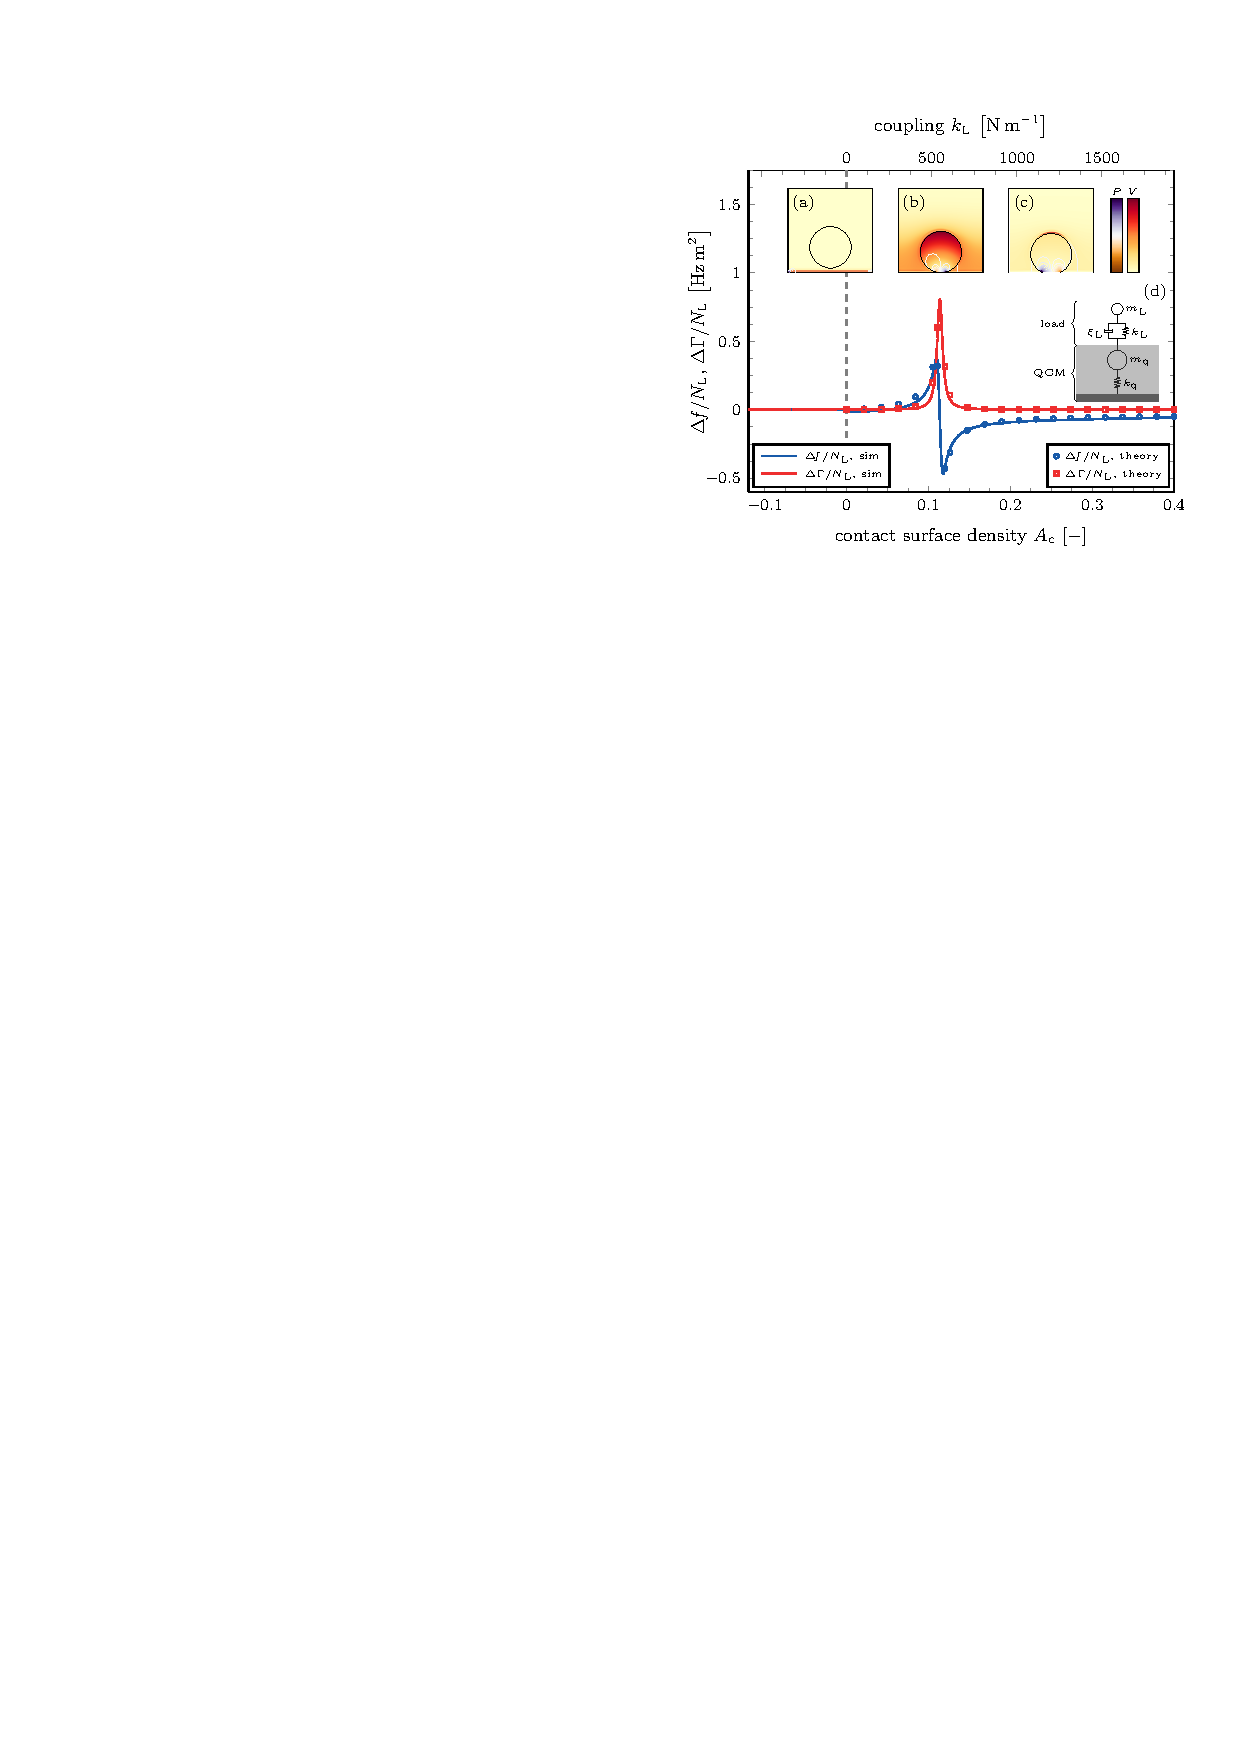
\includegraphics{figure3.pdf}
  \caption{%
    Simulation of the CF-QCM behavior.
    Finite element simulation for a \SI{10}{\micro\meter} polystyrene
    sphere (cylinder in 2D) as a function of contact surface density
    $A_\mathrm{c}$.  Negative values of $A_\mathrm{c}$ indicate positive
    separation from the surface.  Discussion in the text. (a-c): Density plot
    of the pressure $P$ and velocity $U$ distributions. Units are normalized.
    Note that in all situations with finite contact radius,
    stress is annularly distributed around the edge of the contact as per the
    Mindlin model~\cite{kumacheva1998interfacial}.
    (main plot): Shifts in $\df$ and $\dg$.
    (d): Mechanical model based on coupled oscillators. Points on the plot are
    a best fit of the mechanical model to the simulation.}
  \label{fig:lowersphere}
\end{figure}

A plot of the simulated response in frequency and bandwidth for a
\SI{10}{\micro\meter} particle is depicted in \Figure{fig:lowersphere}.
The spheres were modeled as polystyrene with density
$\rho=\SI{1.06}{\gram\per\centi\meter\cubed}$, shear modulus
$|G_\mathrm{L}|=\SI{1.3}{\giga\pascal}$, and loss tangent $\tan \delta =
  0.001$.  The spheres are in water with density
\SI{1.0}{\gram\per\centi\meter\cubed} and viscosity
\SI{1.0}{\milli\pascal\second}.  \linelabel{line:dfdgshiftx}The shifts in $\df$ and $\dg$ are plotted
as a function of a dimensionless contact surface density $A_\mathrm{c}$,
defined as the contact area of the sample per unit area on the oscillating
boundary.

\linelabel{line:closely}The behavior of the simulation closely matches
experimental observations.  As the sphere approaches and makes (weak)
contact with the oscillating boundary, a \textit{positive} shift in both
frequency and bandwidth is observed.  As the contact radius increases, the
sphere becomes more strongly coupled to the boundary. The amount of energy
dissipated into the particle increases until $\dg$ reaches a maximum and
$\df$ experiences a zero crossing.  The limiting case sees a rigid
attachment and the common \textit{negative} frequency shift proportional to
mass adsorption takes hold.
% say here and in the supplement that the velocity component has some phase
% thing

\linelabel{line:twoaspects}There are two aspects of the simulation that deserve additional
consideration:
\begin{inparaenum}[(1)]
  \item positive shifts in $\df$ and $\dg$ begin
  before physical contact with the oscillating boundary and
  \item for smaller particles $\dg>\df$ while for
  larger particles $\df>\dg$.
\end{inparaenum}
The experiment shows the same behavior, as evidenced in
\Table{tbl:particlesize}.  We note however that the procedure of truncation
and its interpretation as finite contact radius in the framework of contact
mechanics utilized here on discrete objects are more accurate for larger
particles (\SI{10}{\micro\meter}, as shown in \Figure{fig:lowersphere})
than smaller ones.  We explain this in the following way.
\linelabel{line:dvlo}It is known in
the context of DVLO theory~\cite{israelachvili2011intermolecular} that a
micron-sized polystyrene sphere in water near a similarly charged gold
surface will experience a repulsive force due to electrostatic double-layer
effects~\cite{alexander1987hydrodynamic}~\cite{flicker1993quantifying}.
The balance between this and the gravitational force determines the height
at which the particle will be at equilibrium above the surface.  For the
relevant material
parameters~\cite{israelachvili2011intermolecular}~\cite{sharma1992factors}
we find that, even at \SI{90}{g}, the smaller \num{1} and
\SI{2}{\micro\meter} particles never make contact with the surface, but
``hover'' at separations of approximately
\SIrange{0.3}{0.15}{\micro\meter}.  At nonzero separations we posit that
the sphere-surface coupling, being mediated by a viscous liquid, will be
dominated by loss, hence $\dg>\df$.  On the other hand, larger particles
($\sim\SI{10}{\micro\meter}$ and above) with significant mass will overcome
the double-layer forces and make contact with the \gls{qcm} through a finite
contact radius.  In this case the coupling losses decrease and $\df>\dg$.

%\subsection*{Mechanical Model}
%\label{sec:mechanicalmodel}
Without mention of the actual physics of the coupling, we observe that the
finite element simulation, as well as the experimental data, follow a simple
mechanical model based on coupled
oscillators~\cite{dybwad1985sensitive}~\cite{olsson2012probing}.  The
arrangement of this mass-spring-dashpot mechanical model is shown in
\Figure{fig:lowersphere}(d).  \linelabel{line:qcmresonance}Here, the resonance of the quartz crystal
$\omegaq^2=\kq/\mq$ is coupled to a sample load with mass $\ml$ though a
parallel spring $\kl$ and dashpot $\xil$ (Voigt
model~\cite{sips1950mechanical}).  \linelabel{line:actualspring}Note that $\kl$ is not an actual spring; it
is simply a coupling strength between two oscillators.  The same is true for
$\xil$.  $\ml$ is an actual mass, though in this model it represents a
Sauerbrey mass uncorrected for viscoelastic properties.

Using the small load approximation, the response of the system as a
function of its coupling $\kl$ can be expressed
as~\cite{steinem2007piezoelectric}
\begin{equation}
  \frac{\df + \mi \dg}{f_\mathrm{F}} = \frac{N_\mathrm{L}}{\pi
    \mathrm{Z}_\mathrm{q}}
  \frac{\ml \omegaq \left( \kl + \mi
    \omegaq \xil\right) }
  {\ml \omegaq^2 - \left(\kl + \mi
    \omegaq \xil\right)}
  \label{eqn:mastereq}
\end{equation}
where $\mathrm{Z}_\mathrm{q}$ is the acoustic impedance of AT cut quartz,
$f_\mathrm{F}$ is the fundamental frequency of the resonator, and
$N_\mathrm{L}$ is a surface density (number per unit area) for discrete
loads.  \linelabel{line:klfinite}\Equation{eqn:mastereq} as a function of $\kl$ reproduces the
response of the finite element simulation in \Figure{fig:lowersphere},
which is a function of contact surface density $A_\mathrm{c}$ (or in
un-normalized terms the contact radius $r_\mathrm{c}$).  A best-fit comparison to
the finite element simulation is shown as points in conjunction with the simulation
in \Figure{fig:lowersphere}.  See Supplementary Note 3.

\linelabel{line:limitsx}The mechanical model has two important limits as a function of the contact
stiffness, $\kl$, known as \textit{strong} and \textit{weak}
coupling.  These limits occur to the left and right of a zero crossing in $\df$ at
$k_\mathrm{zc}=\omegaq^2 \ml$.

\vspace{-\baselineskip}
\vspace{-\parskip}
\begin{align}
  \frac{\df}{f_\mathrm{F}} & =
  \frac{N_\mathrm{L} \kl}
  {\omegaq\pi \mathrm{Z}_\mathrm{q}}
                           & \,                     & \left(\text{weak,}\quad \kl\ll \ml
  \omegaq^2\right)
  \label{eqn:couplinguy1}
  \\
  \frac{\df}{f_\mathrm{F}} & =  -\frac{N_\mathrm{L}
    \ml \omegaq}{\pi Z_\mathrm{q}}
                           & \,                     & \left(\text{strong,}\quad \kl\gg \ml
  \omegaq^2\right)
  \label{eqn:couplinguy2}
\end{align}
\linelabel{line:xilapprox}where we have made the approximation that
$\xil\ll\kl$.~\cite{steinem2007piezoelectric}


\linelabel{line:coupexplain}Strong coupling is identified with mass loading
(Sauerbrey~\cite{sauerbrey1959verwendung} behavior) and a \textit{negative}
frequency shift linearly proportional $\ml$.  This behavior is the
one which is most commonly associated with \gls{qcm} measurements.  Physically
this situation is identified with a coupling rigid enough such that
the particle takes part in the oscillation of the \gls{qcm}.
In the
opposite limit is weak coupling, also called inertial
loading~\cite{dybwad1985sensitive}, and is identified by a \textit{positive}
frequency shift independent of the mass and linearly proportional
to $\kl$.  Here, the coupling is sufficiently weak such that the particle
remains at rest in the labratory frame.  It is ``clamped'' by its own
inertia.~\cite{du2008role}

%This mechanical model fully describes the behavior of the finite element simulations
%for larger ($d\gtrsim\SI{5}{\micro\meter}$) particles, but fails in the
%limit of smaller particles.

\linelabel{line:nanoindentation}Experiments with nanoindentation probes operating on \gls{qcm}. in the gas
phase~\cite{borovsky2001measuring}, where micron-sized spherical tips are
pressed against the sensor surface, have observed the same positive
frequency shift as a function of applied force,  which is identified with
the lateral (sphere-plate) Hertzian spring constant.  We conjecture that
similar behavior will be observed in the liquid phase: the centrifugal load
will primarily act on $\kl$.  We now turn to discussion of how certain
sample parameters can be extracted using this model.

\section*{Discussion}
\label{sec:discussion}
The response of the \gls{qcm} for different load situations under centrifugal
force exhibits a rich and complex set of behavior. Interpretation of all
signals will require experiments beyond the scope of this
manuscript, but we comment on a few examples where our
preliminary data can be predictive within the general model we have set forth.

%\subsection*{Particle Sizing}
%\label{sec:particlesizing}
\begin{figure}[ht]
  \centering
  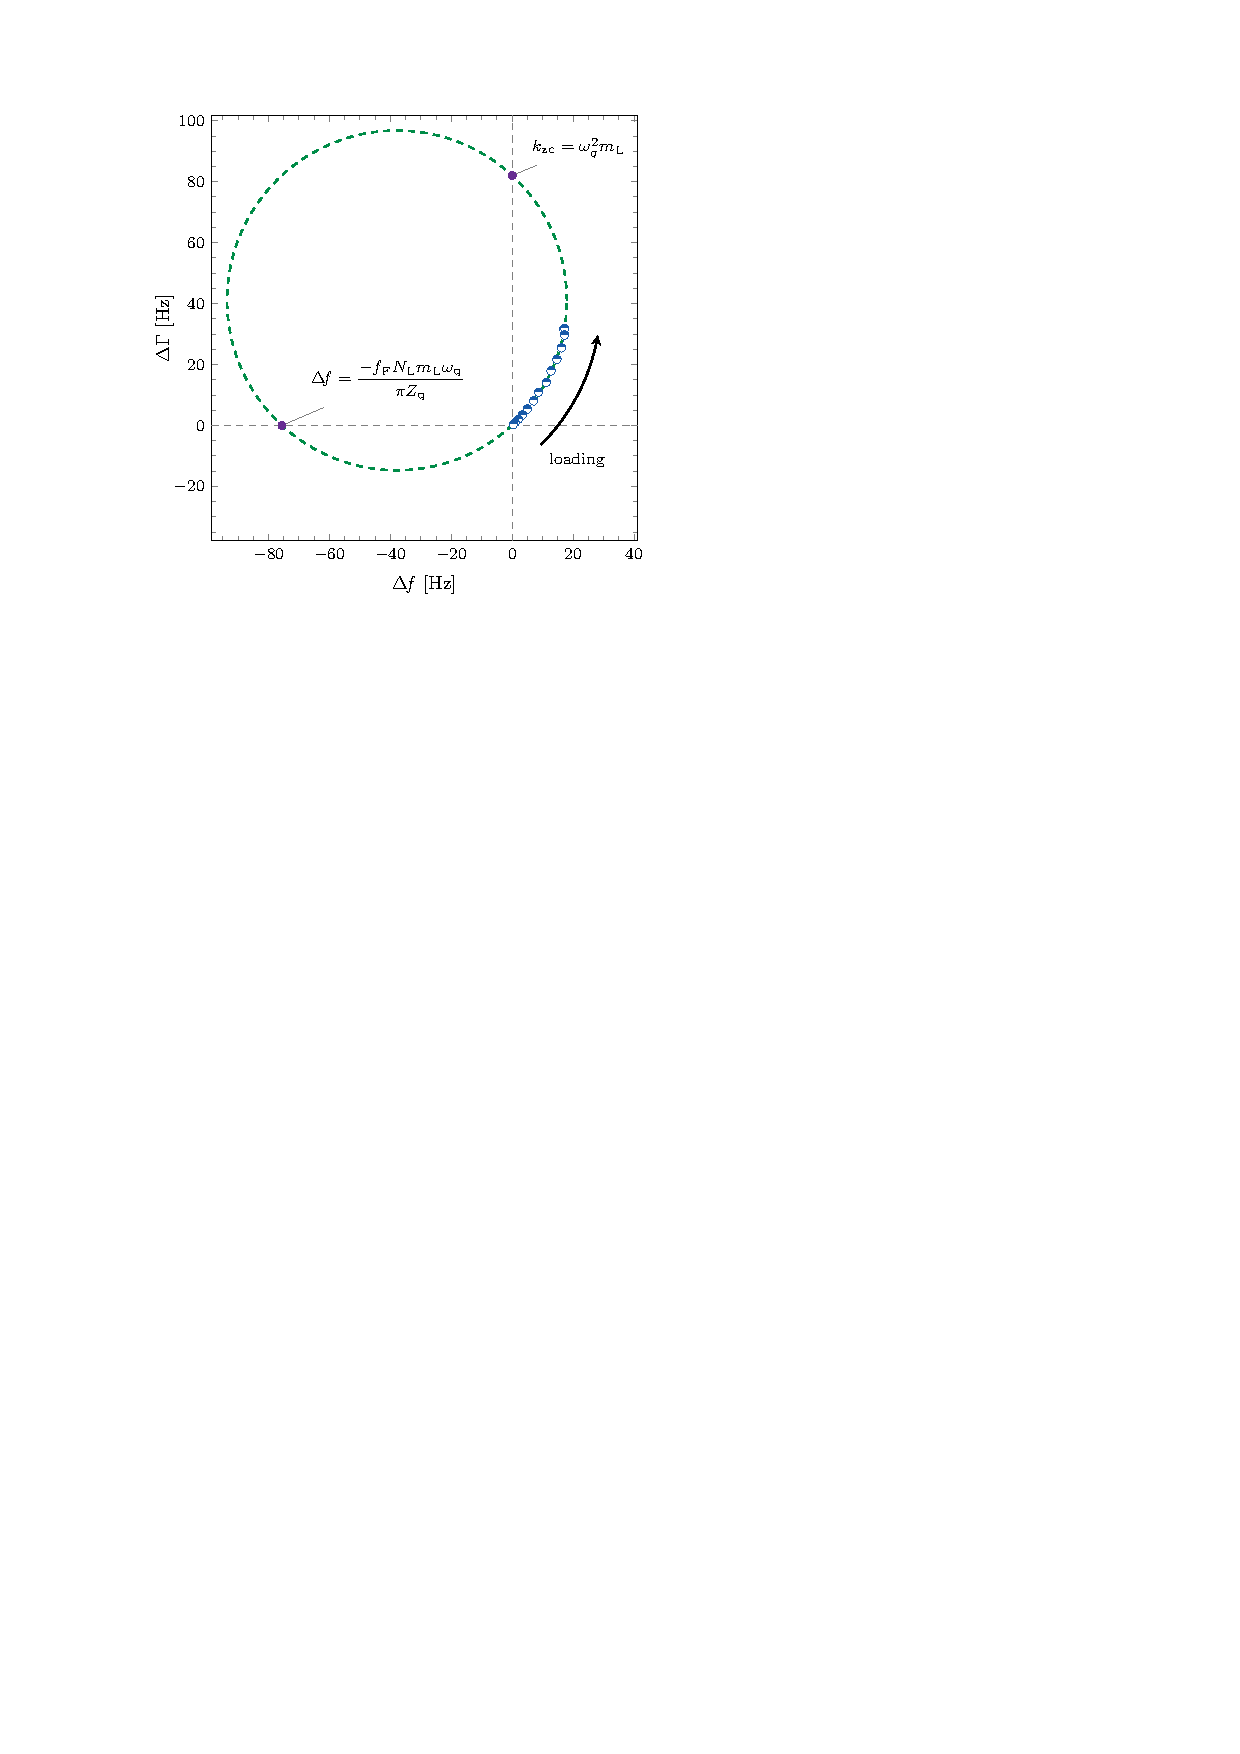
\includegraphics{figure4.pdf}
  \caption{ Particle sizing.  Method for sizing micron-sized particles using the CF-QCM.
    $\df$ versus $\dg$ is plotted parametrically as a function of g-force, and
    the data is fit to a circle.  The point on the circle for which $\dg=0$ and
    $\df<0$ provides an estimate of mass adsorption, and thus particle size.
    Results for particles with diameters $\bar{d}_\mathrm{actual}=1, 2,
      15,\,\mathrm{and}\;\SI{25}{\micro\meter}$ are shown in
    \Table{tbl:particlesizing}.  Fit circle has a radius of \SI{55.77}{\hertz} and
    a center of $(-37.83,41.05) \si{\hertz}$. }
  \label{fig:circlefit}
\end{figure}

\linelabel{line:coupledoscillator}The coupled oscillator model (\Equation{eqn:mastereq}), when analyzed for
samples of free particles (\Figure{fig:expsetup}(b),
\Figure{fig:loadplot}(c), and \Table{tbl:particlesize}), suggests an avenue
to allow \gls{qcm}. to determine the size of large micron-sized particles in the
liquid phase.  Thus far this has only been possible with nanometer-sized
particles which lie within the \gls{qcm}['s] shear acoustic
wave.~\cite{olsson2013using}  \linelabel{line:ifoneplots}If one plots $\df$ versus $\dg$ in
\Equation{eqn:mastereq} as a parametric function of $\kl$, the points are
found to lie on a circle with radius $r_\mathrm{L}$.  In doing so, the physical
mechanism modifying $\kl$ is removed from the problem.
\linelabel{line:fitcircle}If we then fit a
circle to the experimentally observed $\df$-$\dg$ data (plotted
parametrically as a function of g-force), we can extrapolate the behavior
in the strong coupling regime by finding the point at which $\dg=0$ and
$\df<0$.  Knowing $\df$, \Equation{eqn:couplinguy2} can then be inverted to
solve for either number density or particle size/mass.  An example of this
procedure is shown in \Figure{fig:circlefit} using the same data for
\SI{1}{\micro\meter} particles shown in
\Figures{fig:expsetup}{fig:loadplot}.  Inset is a table for the same
predictions done for particles with known diameter
$\bar{d}_\mathrm{actual}=1, 2, 15,\,\mathrm{and}\;\SI{25}{\micro\meter}$.
In all cases the surface density was known and the diameter
$\bar{d}_\text{predicted}$ was derived from the mass $\ml$, found by
inverting \Equation{eqn:couplinguy2}.  The results are surprisingly accurate
despite the exploratory nature of the instrument's construction, which
illustrates the robustness of this unique methodology that CF-QCM
provides.
\linelabel{line:alsobemen}It should also be mentioned that with knowledge of the way in which the
g-force modifies $\kl$, the frequency zero crossing at
$k_\mathrm{zc}=\omegaq^2\ml$ can be used to determine the mass $\ml$
without knowledge of the number density $N_\mathrm{L}$.
\begin{table}[ht]
  \centering
  Particle Sizing\\
  \begin{tabularx}{80pt}{XX}
    \toprule
    $\bar{d}_\mathrm{actual}$ & $\bar{d}_\mathrm{predicted}$ \\
    \midrule
    $1.07^p$                  & \num{1.23+-0.23}             \\
    $1.89^m$                  & \num{1.84+-0.06}             \\
    $15.0^p$                  & \num{13.8+-1.3}              \\
    $24.8^p$                  & \num{22.6+-4.6}              \\
    \bottomrule
  \end{tabularx}
  \caption{Results of the particle sizing method applied to particles with diameters
    $\bar{d}_\mathrm{actual}=1, 2, 15,\,\mathrm{and}\;\SI{25}{\micro\meter}$.}
  \label{tbl:particlesizing}
\end{table}
%\subsection*{Sample Viscoelasticity}
%\label{sec:sampleviscoelasticity}
\linelabel{line:viscosensitive}Finally, we comment on the potential of the CF-QCM technique to be
sensitive to different viscoelastic properties of discrete samples.  While
the mechanical properties seen in biomaterials spans an enormous
range~\cite{meyers2008biological}, we choose three general categories to
highlight potentially interesting sensor responses.  As per
\Figure{fig:multisweep} these are: cells~\cite{li2008thickness}, agarose
microparticles~\cite{li2011surface}~\cite{patra2009viscoelastic}, and
protein microcrystals~\cite{zamiri2009modeling}.  Each is treated in the
finite element simulation as a discrete sphere, with complex shear modulus
$G_\mathrm{L}=G_\mathrm{L}'+G_\mathrm{L}''$, where $G_\mathrm{L}'$ is the
storage modulus related to elasticity, and $G_\mathrm{L}''$ is the loss
modulus related to viscosity.  $G_\mathrm{L}$ is related to viscosity
$\eta_\mathrm{L}$ by $\eta_\mathrm{L}=G_\mathrm{L}/(\mi\omegaq)$.  The
shifts in frequency $\df$ and bandwidth $\dg$ are again plotted as a function of
the dimensionless contact surface density $A_\mathrm{c}$.
\linelabel{line:fictitous}A fictitious negative $A_\mathrm{c}$
is identified with a finite separation distance from the
simulated \gls{qcm} surface.  In all cases the coverage ratio was
\SI{50}{\percent}, and furthermore \linelabel{line:assumekl}we assume that centrifugal force will act to
``push'' the sample into the \gls{qcm} surface, increasing $A_\mathrm{c}$ and
thus the rigidity of its contact with the \gls{qcm}.
\begin{figure}[ht]
  \centering
  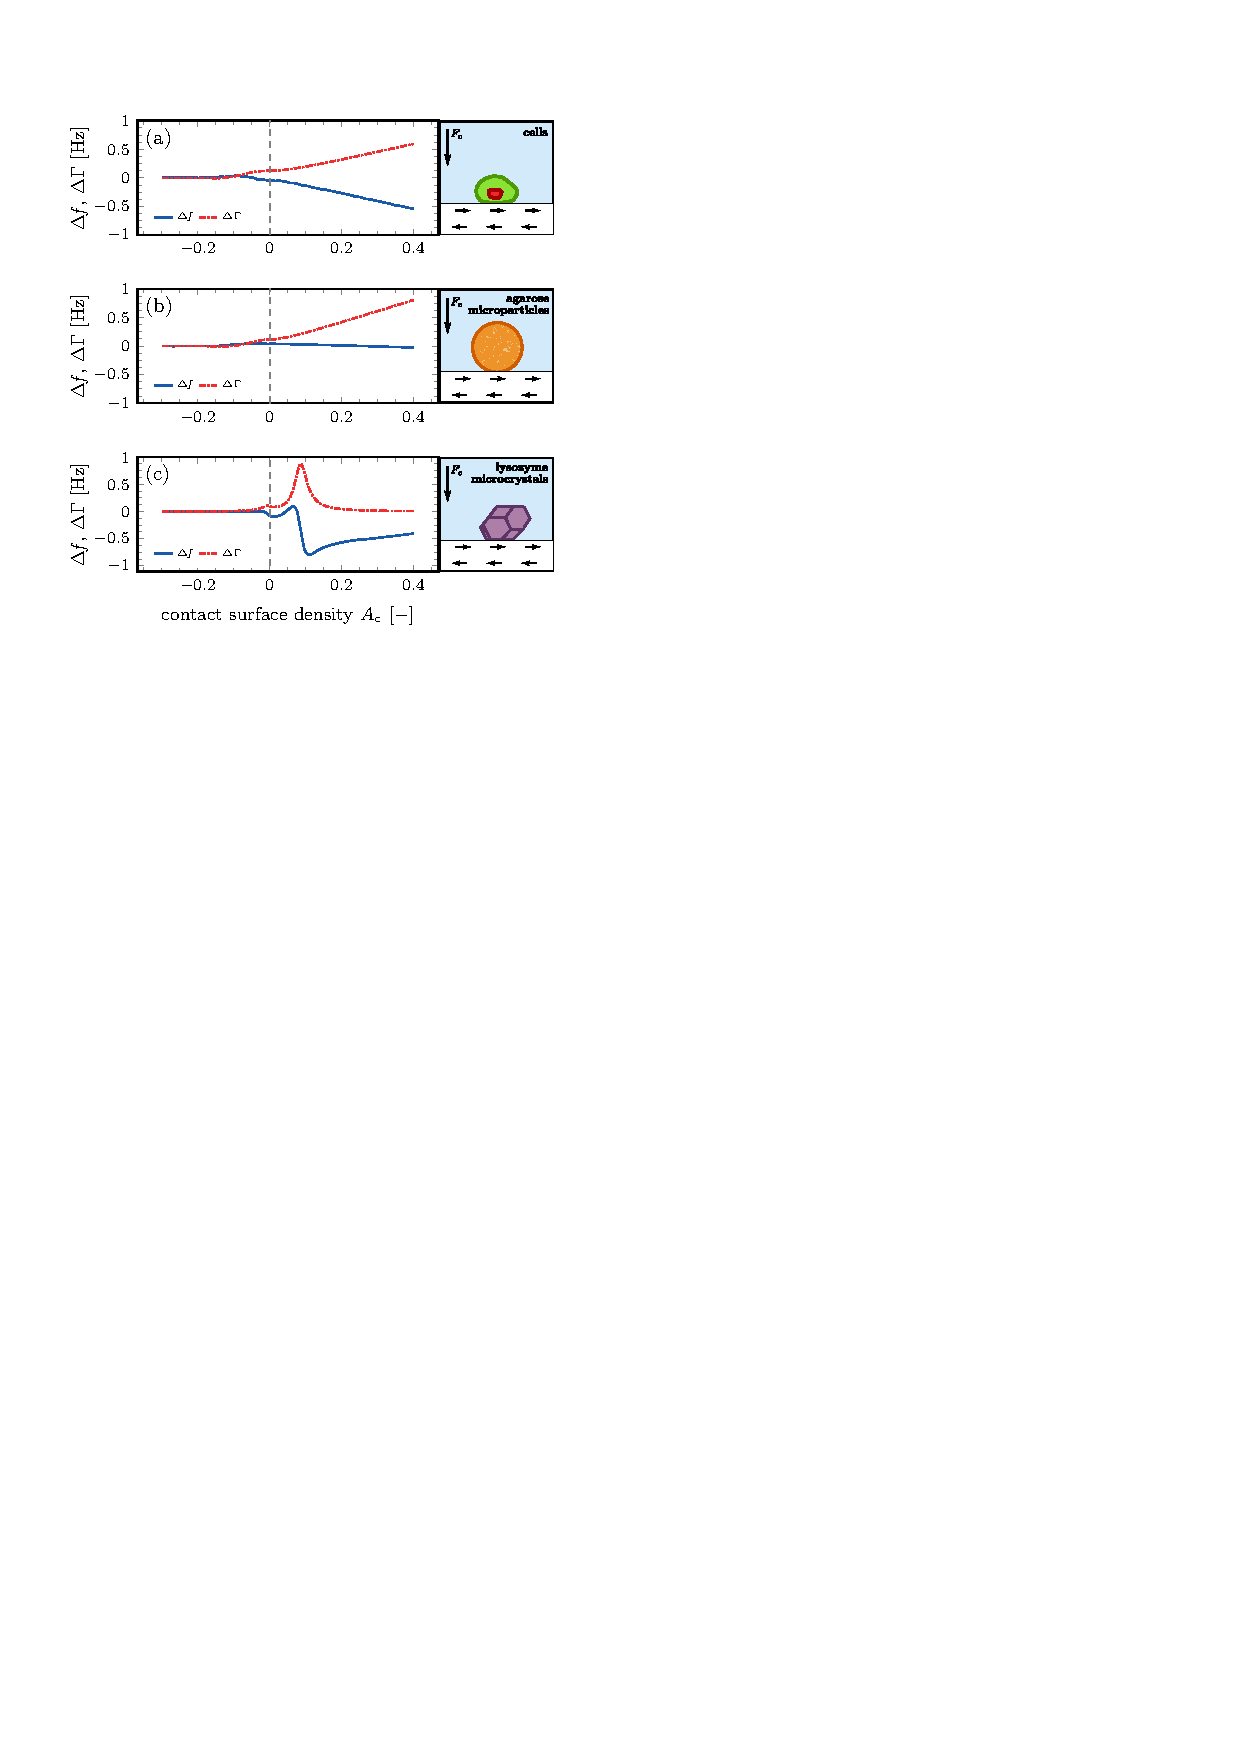
\includegraphics{figure5.pdf}
  \caption{Simulated response for different materials.  Finite element simulation of normalized $\df$ and $\dg$ for three
    categories of samples as a function of contact surface density,
    $A_\mathrm{c}$.
    Negative values indicate the sample has not made contact with the sensor
    surface.
    The samples are (a) cells, $G_\mathrm{L}=\SI{10+50i}{\kilo\pascal}$, (b)
    agarose microparticles, $G_\mathrm{L}=\SI{78+78i}{\kilo\pascal}$ and (c) lysozyme
    microcrystals, $G_\mathrm{L}=\SI{0.659+0.235i}{\giga\pascal}$.  }
  \label{fig:multisweep}
\end{figure}

As can be seen, the simulated response of the CF-QCM is markedly different
in each case. Cells, shown in \Figure{fig:multisweep}(a), are assigned a
shear modulus of $G_\mathrm{L}=\SI{10+50i}{\kilo\pascal}$ and density
$\rho_\mathrm{L}$ equal to the surrounding liquid medium.  The high loss
modulus and low storage modulus predict the cell will exhibit shifts
characteristic of a viscous fluid.  \linelabel{line:viscosens2}Likewise, the simulation shows $\df$
and $\dg$ decrease and increase linearly proportional to the contact
parameter, beginning before physical contact occurs.  The proportionality
is a simple function of the shear modulus and density in the
semi-infinite approximation~\cite{flanigan2000contact}~\cite{kanazawa1985frequency}
\begin{equation}
  \frac{\df+\mi\dg}{f_\mathrm{F}}=\frac{\mi}{\pi Z_\mathrm{q}}\sqrt{\rho_\mathrm{L} G_\mathrm{L}}
  \left(A_\mathrm{c}\right)
\end{equation}
Cells in and of
themselves span a large range of viscoelastic properties which have been
demonstrated to be predictive for diseases such as
cancer~\cite{rebelo2013comparison}.  \linelabel{line:ifoneknows}If one knows the way with which
$A_\mathrm{c}$ is modulated by an applied force (e.g.\ viscoelastic
compliance), linear fitting to
the CF-QCM response will recover $G_\mathrm{L}$ or $\rho_\mathrm{L}$.

Next, \Figure{fig:multisweep}(b) shows the simulated response of agarose
microparticles with a complex shear modulus of
$G_\mathrm{L}=\SI{78+78i}{\kilo\pascal}$. Again the density was assumed to
be the same as the surrounding medium.  Similar to the viscous behavior of
cells, $\dg$ decreases linearly with $A_\mathrm{c}$.  In this
sample however, an equally large elastic term, $G'_\mathrm{L}$, precludes
the equally linear decrease in $\df$ seen for cells.  Instead, $\df$ increases
slightly before contact and decreases slightly.

At the end of the spectrum, \Figure{fig:multisweep}(c) are lysozyme
microcrystals.  These microcrystals are ``hard'', having been assigned a
complex shear modulus of $G_\mathrm{L}=\SI{0.659+0.235i}{\giga\pascal}$.
The response of these is similar to what we experimentally observe with
polystyrene microparticles ($G_\mathrm{L}=\SI{1.3}{\giga\pascal}$).  When
the microcrystal enters the acoustic evanescent wave, there is an initial
negative shift as the effective viscosity-density product increases.  At
small contact parameters there is a positive shift in $\df$ and $\dg$.
Increasing the contact parameter, $\dg$ sees a maximum and $\df$ a zero
crossing.  As the microcrystal becomes strongly coupled to the \gls{qcm}. the
familiar negative $\df$ is recovered which, as in \Figure{fig:circlefit},
can be used to determine the particle size or mass.

%\subsection*{Conclusion}
%\label{sec:conclusion}
We have observed the \gls{qcm} sensorgram under the influence of centrifugal force
for samples such as DNA monolayers, free discrete polystyrene particles,
and particles tethered to the \gls{qcm} electrode with lambda DNA.  We present
simulations and a theoretical framework to interpret the \gls{qcm} signals in the
context of the sample's properties.

The data presented thus far points to a potentially interesting avenue for
the investigation of force on biomolecules using a quartz crystal
microbalance.  In addition to the data discussed, we have also observed
other types of signals in some of our datasets within the overall trend
shown here, which we suspect may be related to ionic
transport~\cite{tolman1911electromotive}~\cite{des1893unpolarisirbare}, the
conformal state of DNA, and nonlinear viscoelastic behavior.  Objects such
as microparticles attached or tethered to a biopolymer on the \gls{qcm} surface
become inertial transducers through which one can extract mechanical and
thermodynamic properties of the macromolecules. Furthermore, the technique
is applicable to microscopic biological objects such as viruses, bacteria,
and cells where measurements of mechanical properties and their changes
have been directly linked to
disease~\cite{merkel1989molecular}~\cite{yeri2009mutation}~\cite{tevet2011friction}.

The enhanced signal for most samples under centrifugal load points to a
interesting avenue of increasing the sensitivity of a state of the art QCM
biosensor.  This is true even with the present state of our instrument,
which is limited to low-g regimes when compared to other commercial
centrifuges. With operation below \SI{90}{g}, we have observed sensitivity
increases corresponding to changes of \SI{10}{\percent} in the
density-viscosity product for viscoelastic loads, and up to a factor of 10
increase in sensitivity for discrete particles.  However, there is no
technical reason why future incarnations could not spin much faster and
considerably clarify the CF-QCM sensogram.  There are also possibilities in
using this platform in other related modalities such as the
nanotribological effects of sliding friction~\cite{krim1991nanotribology}
caused by orienting the crystal at an angle to the applied centrifugal
force, propelling biomolecules across the surface.

\section*{Methods}
\label{sec:materials}
The experimental setup used a \SI{25}{\milli\meter} diameter
\SI{5}{\mega\hertz} gold-coated crystal in combination with an SRS QCM200
PLL-based driver circuit.  On the sensing side of the crystal is a
\SI{125}{\micro\liter} PDMS/glass cell containing the specimen under
investigation.  The cell is made of a thin o-ring of PDMS (Sylgard 184,
10:1 ratio, cured \SI{20}{\minute} at \SI{120}{\celsius})
$\text{OD}=\SI{25}{\milli\meter}$, $\text{ID}=\SI{15.5}{\milli\meter}$ in
contact with the sensing side of the crystal and covered with
\SI{25}{\milli\meter} round N\raisebox{0.25em}{\relsize{-2}\b{o}}~1
cover glass, nominal thickness \SI{0.15}{\milli\meter}.  The non-sensing
side of the crystal remains in air and is isolated from the body of the
centrifuge.  The quartz crystals are always cleaned before use by immersion
in fresh piranha solution (3:1 mixture of \SI{97}{\percent} \ce{H2SO4} and
\SI{30}{\percent} \ce{H2O2}) for \SI{5}{\minute} and rinsing liberally with
pure water.

Free particles (Spherotech SVP-10-5, SVM-15-10, and SVP-200-4), of
different diameters were prepared by diluting a solution of
\SI{30}{\micro\liter} particles in \SI{300}{\micro\liter} \ce{H2O}.  A
\SI{125}{\micro\liter} aliquot of the \SI{300}{\micro\liter} volume was
then placed in the PDMS cell in contact with the sensing side of the
crystal.  The sensing area was calculated to be
\SI{1.195}{\centi\meter\squared}.  The particles in solution experience a
buoyant force which reduces their apparent mass. The surface density
$N_\mathrm{L}$ was determined by counting the average number of particles
per unit area with a microscope and was found to be within
\SI{20}{\percent} of the value predicted by the volume concentration.

For experiments involving oligos, the crystals were first immersed in a
\SI{1}{\micro\textsc{M}} solution of thiolated oligos (5'-ThioMC6-TTT TTT
TTT CAC TAA AGT TCT TAC CCA TCG CCC-3') in a \SI{1}{\textsc{M}} potassium
phosphate buffer, \SI{0.5}{\textsc{M}} \ce{KH2PO4}, pH 3.8 for
\SI{1}{\hour}.  Following, immersion in \SI{1}{\milli\textsc{M}}
6-Mercapto-1-hexanol (MCH) was used to block residual reactive sites on the
gold electrode.  After rinsing, attachment to the prepared particles was
done in STE buffer: \SI{1}{\textsc{M}} \ce{NaCl} with
\SI{10}{\milli\textsc{M}} Tris buffer, pH 7.4 and \SI{1}{\milli\textsc{M}}
EDTA\@.  A complementary strand (5'-biotin-CT CAC TAT AGG GCG ATG GGT AAG
AAC TTT AGT-3') was attached to the streptavidin-coated particles.  The
particles were first washed two times by alliquoting a
\SI{100}{\micro\liter} base solution of particles in \SI{100}{\micro\liter}
STE buffer, \SI{5000}{RPM} for \SI{3}{\minute} and decanting the
supernatant.  The particles were resuspended in \SI{20}{\micro\liter} of
STE buffer and \SI{10}{\micro\gram} of oligos were added.  The mixture was
incubated \SI{15}{\minute} at room temperature under slow vortexing, then
washed again and resuspended in \SI{100}{\micro\liter} STE buffer.  The
oligo-attached particle suspension was allowed to attach to the gold
surface for \SI{15}{\minute} before spinning.

Lambda DNAs were prepared by combining \SI{50}{\micro\liter} of lambda DNA
at \SI{500}{\micro\gram\per\milli\liter}, \SI{5.5}{\micro\liter} of 10x T4
ligase, and \SI{0.5}{\micro\liter} of diluted \SI{10}{\micro\textsc{M}}
thiolated linker oligonucleotide and heating to \SI{70}{\celsius} for
\SI{5}{\minute}.  The suspension was left to cool to room temperature as
the litigation of the oligos to the DNA COS ends occured. Once the mixture
was at room temperature, \SI{15}{\micro\liter} 10x ligase buffer,
\SI{127}{\micro\liter} \ce{H2O}, and \SI{2}{\micro\liter} T4 DNA ligase was
added to the annealed linker.  The reaction was allowed to proceed at room
temperature for \SI{3}{\hour}.

\section*{Acknowledgments}
\label{sec:acknowledgements}
The authors acknowledge the work of D\@.~Schaak in preparing and determining
the protocols for the biological samples and C\@.~Stokes for building the
supporting electronics and data acquisition hardware.

This work was supported by the Max Plank Society, the International Max
Planck Research School for the Science of Light, and the Rowland Institute
at Harvard University.

\section*{Author contributions}
A.W.\@ carried out the experiments and wrote the manuscript.  Y.S.\@
conceived the idea and supervised the experiment.  F.V., Y.S., and
A.W.\@ planned the experiment.  F.V.\@ supervised the data analysis.

\section*{Competing financial interests}
The authors declare no competing financial interests.

% Used to generate bibiography.  Include the *.bbl file here directly.
\nocite{hussain2005ots}
\nocite{gottschling2000detection}
\nocite{snellings2001response}
\nocite{srsqcm200manual}
\nocite{su2005comparison}
\nocite{peh2007understanding}

\bibliographystyle{unsrt}
%\bibliography{bibliography}

\begin{thebibliography}{10}

  \bibitem{felsenfeld1992chromatin}
  Gary Felsenfeld.
  \newblock Chromatin as an essential part of the transcriptional mechanism.
  \newblock {\em Nature}, 355:219--224, 1992.

  \bibitem{cui2000pulling}
  Yujia Cui and Carlos Bustamante.
  \newblock Pulling a single chromatin fiber reveals the forces that maintain its
  higher-order structure.
  \newblock {\em Proceedings of the National Academy of Sciences},
  97(1):127--132, 2000.

  \bibitem{larson2012trigger}
  Matthew~H Larson, Jing Zhou, Craig~D Kaplan, Murali Palangat, Roger~D Kornberg,
  Robert Landick, and Steven~M Block.
  \newblock Trigger loop dynamics mediate the balance between the transcriptional
  fidelity and speed of {RNA} polymerase {II}.
  \newblock {\em Proceedings of the National Academy of Sciences},
  109(17):6555--6560, 2012.

  \bibitem{marko1995stretching}
  John~F Marko and Eric~D Siggia.
  \newblock Stretching {DNA}.
  \newblock {\em Macromolecules}, 28(26):8759--8770, 1995.

  \bibitem{suda2001origin}
  Hitoshi Suda.
  \newblock Origin of friction derived from rupture dynamics.
  \newblock {\em Langmuir}, 17(20):6045--6047, 2001.

  \bibitem{bormuth2009protein}
  Volker Bormuth, Vladimir Varga, Jonathon Howard, and Erik Sch{\"a}ffer.
  \newblock Protein friction limits diffusive and directed movements of kinesin
  motors on microtubules.
  \newblock {\em Science}, 325(5942):870--873, 2009.

  \bibitem{asbury2003kinesin}
  Charles~L Asbury, Adrian~N Fehr, and Steven~M Block.
  \newblock Kinesin moves by an asymmetric hand-over-hand mechanism.
  \newblock {\em Science}, 302(5653):2130--2134, 2003.

  \bibitem{sauerbrey1959verwendung}
  G{\"u}nter Sauerbrey.
  \newblock Verwendung von {S}chwingquarzen zur {W}{\"a}gung d{\"u}nner
  {S}chichten und zur {M}ikrow{\"a}gung.
  \newblock {\em Zeitschrift f{\"u}r Physik}, 155(2):206--222, 1959.

  \bibitem{kanazawa1985frequency}
  K.~Keiji Kanazawa and Joseph~G. Gordon.
  \newblock Frequency of a quartz microbalance in contact with liquid.
  \newblock {\em Analytical Chemistry}, 57(8):1770--1771, 1985.

  \bibitem{johannsman2007contacts}
  Diethelm Johannsmann.
  \newblock {\em Studies of Contact Mechanics with the {QCM}}, pages 151--170.
  \newblock Springer, 2007.

  \bibitem{marx2003quartz}
  Kenneth~A Marx.
  \newblock Quartz crystal microbalance: a useful tool for studying thin polymer
  films and complex biomolecular systems at the solution-surface interface.
  \newblock {\em Biomacromolecules}, 4(5):1099--1120, 2003.

  \bibitem{borovsky2001measuring}
  B~Borovsky, J~Krim, SA~{Syed Asif}, and KJ~Wahl.
  \newblock Measuring nanomechanical properties of a dynamic contact using an
  indenter probe and quartz crystal microbalance.
  \newblock {\em Journal of Applied Physics}, 90(12):6391--6396, 2001.

  \bibitem{richter2003pathways}
  Ralf Richter, Anneke Mukhopadhyay, and Alain Brisson.
  \newblock Pathways of lipid vesicle deposition on solid surfaces: a combined
    {QCM-D} and {AFM} study.
  \newblock {\em Biophysical Journal}, 85(5):3035--3047, 2003.

  \bibitem{fawcett2004evidence}
  Newton~C Fawcett, Richard~D Craven, Ping Zhang, and Jeffrey~A Evans.
  \newblock Evidence for gravity's influence on molecules at a solid-solution
  interface.
  \newblock {\em Langmuir}, 20(16):6651--6657, 2004.

  \bibitem{yoshimoto2002effect}
  Minoru Yoshimoto and Shigeru Kurosawa.
  \newblock Effect of immersion angle of a one-face sealed quartz crystal
  microbalance in liquid.
  \newblock {\em Analytical Chemistry}, 74(16):4306--4309, 2002.

  \bibitem{filler1988acceleration}
  Raymond~L Filler.
  \newblock The acceleration sensitivity of quartz crystal oscillators: a review.
  \newblock {\em Ultrasonics, Ferroelectrics and Frequency Control, IEEE
    Transactions on}, 35(3):297--305, 1988.

  \bibitem{arnau2002circuit}
  A~Arnau, T~Sogorb, and Y~Jim{\'e}nez.
  \newblock Circuit for continuous motional series resonant frequency and
  motional resistance monitoring of quartz crystal resonators by parallel
  capacitance compensation.
  \newblock {\em Review of Scientific Instruments}, 73(7):2724--2737, 2002.

  \bibitem{geelhood2002transient}
  SJ~Geelhood, CW~Frank, and K~Kanazawa.
  \newblock Transient quartz crystal microbalance behaviors compared.
  \newblock {\em Journal of the Electrochemical Society}, 149(1):H33--H38, 2002.

  \bibitem{valdois2794influence}
  M.~Valdois, J.~Besson, and J.-J. Gagnepain.
  \newblock Influence of environment conditions on a quartz resonator.
  \newblock In {\em 28th Annual Symposium on Frequency Control. 1974}, pages
  19--32, 1974.

  \bibitem{tsortos2008shear}
  Achilleas Tsortos, George Papadakis, and Electra Gizeli.
  \newblock Shear acoustic wave biosensor for detecting {DNA} intrinsic viscosity
  and conformation: A study with {QCM-D}.
  \newblock {\em Biosensors and Bioelectronics}, 24(4):836--841, 2008.

  \bibitem{encarnaccao2007influence}
  Joao~M Encarna\c{c}ao, Peter Stallinga, and Guilherme~NM Ferreira.
  \newblock Influence of electrolytes in the {QCM} response: Discrimination and
  quantification of the interference to correct microgravimetric data.
  \newblock {\em Biosensors and Bioelectronics}, 22(7):1351--1358, 2007.

  \bibitem{lin1995role}
  Zuxuan Lin and Michael~D Ward.
  \newblock The role of longitudinal waves in quartz crystal microbalance
  applications in liquids.
  \newblock {\em Analytical Chemistry}, 67(4):685--693, 1995.

  \bibitem{yoshimoto2006characteristics}
  Minoru Yoshimoto, Shin Tokimura, and Shigeru Kurosawa.
  \newblock Characteristics of the series resonant-frequency shift of a quartz
  crystal microbalance in electrolyte solutions.
  \newblock {\em Analyst}, 131(10):1175--1182, 2006.

  \bibitem{tolman1911electromotive}
  Richard~C Tolman.
  \newblock The electromotive force produced in solutions by centrifugal action.
  \newblock {\em Journal of the American Chemical Society}, 33(2):121--147, 1911.

  \bibitem{des1893unpolarisirbare}
  Th. {Des Coudres}.
  \newblock Unpolarisirbare electrolytische {Z}ellen unter dem {E}influsse der
    {C}entrifugalkraft.
  \newblock {\em Annalen der Physik}, 285(6):284--294, 1893.

  \bibitem{zhang2002insulating}
  Y.~Zhang, R.~H. Austin, J.~Kraeft, E.~C. Cox, and N.~P. Ong.
  \newblock Insulating behavior of $\lambda$-{DNA} on the micron scale.
  \newblock {\em Physical Review Letters}, 89:198102, Oct 2002.

  \bibitem{kumacheva1998interfacial}
  E~Kumacheva.
  \newblock Interfacial friction measurement in surface force apparatus.
  \newblock {\em Progress in Surface Science}, 58(2):75--120, 1998.

  \bibitem{israelachvili2011intermolecular}
  Jacob~N Israelachvili.
  \newblock {\em Intermolecular and surface forces: revised third edition}.
  \newblock Academic Press, 2011.

  \bibitem{alexander1987hydrodynamic}
  Barbara~M Alexander and Dennis~C Prieve.
  \newblock A hydrodynamic technique for measurement of colloidal forces.
  \newblock {\em Langmuir}, 3(5):788--795, 1987.

  \bibitem{flicker1993quantifying}
  Scott~G Flicker, Jennifer~L Tipa, and Stacy~G Bike.
  \newblock Quantifying double-layer repulsion between a colloidal sphere and a
  glass plate using total internal reflection microscopy.
  \newblock {\em Journal of Colloid and Interface Science}, 158(2):317--325,
  1993.

  \bibitem{sharma1992factors}
  Mukul~M Sharma, Habib Chamoun, DSH Sarma, and Robert~S Schechter.
  \newblock Factors controlling the hydrodynamic detachment of particles from
  surfaces.
  \newblock {\em Journal of Colloid and Interface Science}, 149(1):121--134,
  1992.

  \bibitem{dybwad1985sensitive}
  GL~Dybwad.
  \newblock A sensitive new method for the determination of adhesive bonding
  between a particle and a substrate.
  \newblock {\em Journal of Applied Physics}, 58:2789, 1985.

  \bibitem{olsson2012probing}
  Adam~LJ Olsson, Henny~C van~der Mei, Diethelm Johannsmann, Henk~J Busscher, and
  Prashant~K Sharma.
  \newblock Probing colloid--substratum contact stiffness by acoustic sensing in
  a liquid phase.
  \newblock {\em Analytical Chemistry}, 84(10):4504--4512, 2012.

  \bibitem{sips1950mechanical}
  Robert Sips.
  \newblock Mechanical behavior of viscoelastic substances.
  \newblock {\em Journal of Polymer Science}, 5(1):69--89, 1950.

  \bibitem{steinem2007piezoelectric}
  Claudia Steinem, Andreas Janshoff, and Matthew~A Cooper.
  \newblock {\em Piezoelectric sensors}, volume~5.
  \newblock Springer, 2007.

  \bibitem{du2008role}
  Binyang Du, Alexander~Martin K{\"o}nig, and Diethelm Johannsmann.
  \newblock On the role of capillary instabilities in the sandcastle effect.
  \newblock {\em New Journal of Physics}, 10(5):053014, 2008.

  \bibitem{olsson2013using}
  Adam~LJ Olsson, Ivan~R Quevedo, Danqing He, Mohan Basnet, and Nathalie
  Tufenkji.
  \newblock Using the quartz crystal microbalance with dissipation monitoring to
  evaluate the size of nanoparticles deposited on surfaces.
  \newblock {\em ACS Nano}, 7(9):7833--7843, 2013.

  \bibitem{meyers2008biological}
  Marc~Andr{\'e} Meyers, Po-Yu Chen, Albert Yu-Min Lin, and Yasuaki Seki.
  \newblock Biological materials: structure and mechanical properties.
  \newblock {\em Progress in Materials Science}, 53(1):1--206, 2008.

  \bibitem{li2008thickness}
  Fang Li, James H-C Wang, and Qing-Ming Wang.
  \newblock Thickness shear mode acoustic wave sensors for characterizing the
  viscoelastic properties of cell monolayer.
  \newblock {\em Sensors and Actuators B: Chemical}, 128(2):399--406, 2008.

  \bibitem{li2011surface}
  Ang Li, Edmondo~M Benetti, Davide Tranchida, Jarred~N Clasohm, Holger
  Sch{\"o}nherr, and Nicholas~D Spencer.
  \newblock Surface-grafted, covalently cross-linked hydrogel brushes with
  tunable interfacial and bulk properties.
  \newblock {\em Macromolecules}, 44(13):5344--5351, 2011.

  \bibitem{patra2009viscoelastic}
  Leena Patra and Ryan Toomey.
  \newblock Viscoelastic response of photo-cross-linked poly
  (n-isopropylacrylamide) coatings by {QCM-D}.
  \newblock {\em Langmuir}, 26(7):5202--5207, 2009.

  \bibitem{zamiri2009modeling}
  Amir Zamiri and Suvranu De.
  \newblock Modeling the mechanical response of tetragonal lysozyme crystals.
  \newblock {\em Langmuir}, 26(6):4251--4257, 2009.

  \bibitem{flanigan2000contact}
  Cynthia~M Flanigan, Manishi Desai, and Kenneth~R Shull.
  \newblock Contact mechanics studies with the quartz crystal microbalance.
  \newblock {\em Langmuir}, 16(25):9825--9829, 2000.

  \bibitem{rebelo2013comparison}
  LM~Rebelo, JS~de~Sousa, J~Mendes~Filho, and M~Radmacher.
  \newblock Comparison of the viscoelastic properties of cells from different
  kidney cancer phenotypes measured with atomic force microscopy.
  \newblock {\em Nanotechnology}, 24(5):055102, 2013.

  \bibitem{merkel1989molecular}
  R~Merkel, E~Sackmann, and E~Evans.
  \newblock Molecular friction and epitactic coupling between monolayers in
  supported bilayers.
  \newblock {\em Journal de Physique}, 50(12):1535--1555, 1989.

  \bibitem{yeri2009mutation}
  Ashish~S Yeri, Lizeng Gao, and Di~Gao.
  \newblock Mutation screening based on the mechanical properties of {DNA}
  molecules tethered to a solid surface.
  \newblock {\em The Journal of Physical Chemistry B}, 114(2):1064--1068, 2009.

  \bibitem{tevet2011friction}
  Ofer Tevet, Palle Von-Huth, Ronit Popovitz-Biro, Rita Rosentsveig, H~Daniel
  Wagner, and Reshef Tenne.
  \newblock Friction mechanism of individual multilayered nanoparticles.
  \newblock {\em Proceedings of the National Academy of Sciences},
  108(50):19901--19906, 2011.

  \bibitem{krim1991nanotribology}
  J~Krim, DH~Solina, and R~Chiarello.
  \newblock Nanotribology of a kr monolayer: A quartz-crystal microbalance study
  of atomic-scale friction.
  \newblock {\em Physical Review Letters}, 66(2):181--184, 1991.

  \bibitem{hussain2005ots}
  Yazan Hussain, Jacqueline Krim, and Christine Grant.
  \newblock Ots adsorption: A dynamic {QCM} study.
  \newblock {\em Colloids and Surfaces A: Physicochemical and Engineering
    Aspects}, 262(1):81--86, 2005.

  \bibitem{gottschling2000detection}
  Daniel~E Gottschling, Robert~D Grober, and Michael Sailor.
  \newblock Detection of biological warefare agents.
  \newblock 2000.

  \bibitem{snellings2001response}
  Shannon~L Snellings, Jason Fuller, and David~W Paul.
  \newblock Response of a thickness-shear-mode acoustic wave sensor to the
  adsorption of lipoprotein particles.
  \newblock {\em Langmuir}, 17(8):2521--2527, 2001.

  \bibitem{srsqcm200manual}
  Stanford~Research Systems.
  \newblock {\em {QCM200} quartz crystal microbalance digital controller:
    operation and service manual}.
  \newblock 2004.

  \bibitem{su2005comparison}
  Xiaodi Su, Ying-Ju Wu, and Wolfgang Knoll.
  \newblock Comparison of surface plasmon resonance spectroscopy and quartz
  crystal microbalance techniques for studying {DNA} assembly and
  hybridization.
  \newblock {\em Biosensors and Bioelectronics}, 21(5):719--726, 2005.

  \bibitem{peh2007understanding}
  Wendy~YX Peh, Erik Reimhult, Huey~Fang Teh, Jane~S Thomsen, and Xiaodi Su.
  \newblock Understanding ligand binding effects on the conformation of estrogen
  receptor $\alpha$-{DNA} complexes: A combinational quartz crystal
  microbalance with dissipation and surface plasmon resonance study.
  \newblock {\em Biophysical Journal}, 92(12):4415--4423, 2007.

\end{thebibliography}

% Äpfel
\end{document}
